\documentclass[10pt]{beamer}

% Packages
\usepackage{graphicx}
\usepackage{hyperref}
\usepackage{listings}
\usepackage{color}
\usepackage{tikz}
\usepackage{amsmath}
\usepackage{amssymb}
\usepackage{helvet} 
\usepackage{caption}
\usepackage{bookmark}

\usetikzlibrary{positioning}

% Beamer settings
\usetheme{metropolis}
\usecolortheme{default}

% Document settings
\title{TFE25-462: Meeting 7}
\subtitle{Schmidl and Cox Synchronization}
\author{Quentin Prieels}
\date{\today}


\begin{document}

% Title slide
\maketitle

% Table of contents
%\begin{frame}
%\frametitle{Table of contents}
%    \tableofcontents
%\end{frame}

%%%%%%%%%%%%%%%%%%%%%%%%%%%
% PART : Schmidl and Cox %
%%%%%%%%%%%%%%%%%%%%%%%%%%%
\section{Theoretical background}

\begin{frame}
    \frametitle{Schmidl and Cox frame structure}
    The Schmidl and Cox synchronization algorithm is based on the following frame structure:
    \begin{figure}
        \centering
        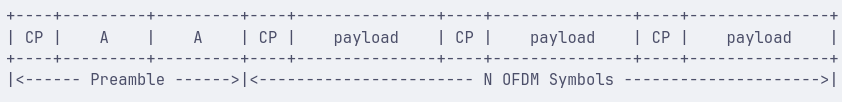
\includegraphics[width=\textwidth]{frame-structure.png}
        \caption{Schmidl and Cox frame structure}
    \end{figure}
    \begin{itemize}
        \item OFDM $0$ symbols on odd subcarriers % impairs
        \item Gives a symmetric symbols in time domain
    \end{itemize}
\end{frame}

\begin{frame}
    \frametitle{Schmidl and Cox synchronization algorithm - basics}
    \begin{itemize}
        \item Calculate the correlation of the received signal with itself shifted by $L$ samples
            $P(d) = \sum_{n=0}^{L-1} r*_{d+m} r_{d+m+L}$
                       calculated as
            \[P(d + 1) = P(d) + r*_{d - L} r_{d} - r*_{d - 2L} r_{d - L}\]
        \item Recieved energy for second the second half-symbols $R(d) = \sum_{n=0}^{L-1} |r(d+m+L)|^2$
            calculated as 
            \[R(d + 1) = R(d) + |r(d)|^2 - |r(d - L)|^2\]
        \item Calculate the metric
            \[M(d) = \frac{|P(d)|^2}{(R(d))^2}\]
    \end{itemize}
    where $r$ is the received signal and $L = K / 2$ with $K$ the number of subcarriers (FFT size). So, in time domain, a symbol has a size of $CP + K = CP + 2L$ samples.
\end{frame}

\frame{
    \frametitle{Schmidl and Cox synchronization algorithm - averaging}
    Moving average window of size $width$:
    \begin{itemize}
        \item The metric $M(d)$ has a plateau of size $CP$ samples
        \item The metric $M(d)$ is averaged over a window of $N$ samples
            \[N(d + 1) = \frac{1}{width} \cdot (N(d) + M(d) - M(d - width)))\]
    \end{itemize}

    Delay introduced:
    \begin{itemize}
        \item M\_delay = $K \cdot M$ (or $2L \cdot M$): introduced by computing the metric
        \item AVG\_delay = $width / 2 \cdot M$: introduced by the moving window
        \item MID\_delay = $CP/2 \cdot M$: the peak of N indicates the middle of the cyclic prefix
    \end{itemize}
    where $M$ is the oversampling factor.
}

\section{Simulation}

\frame{
    \frametitle{Theoretical Simulation}
    \begin{figure}
        \centering
        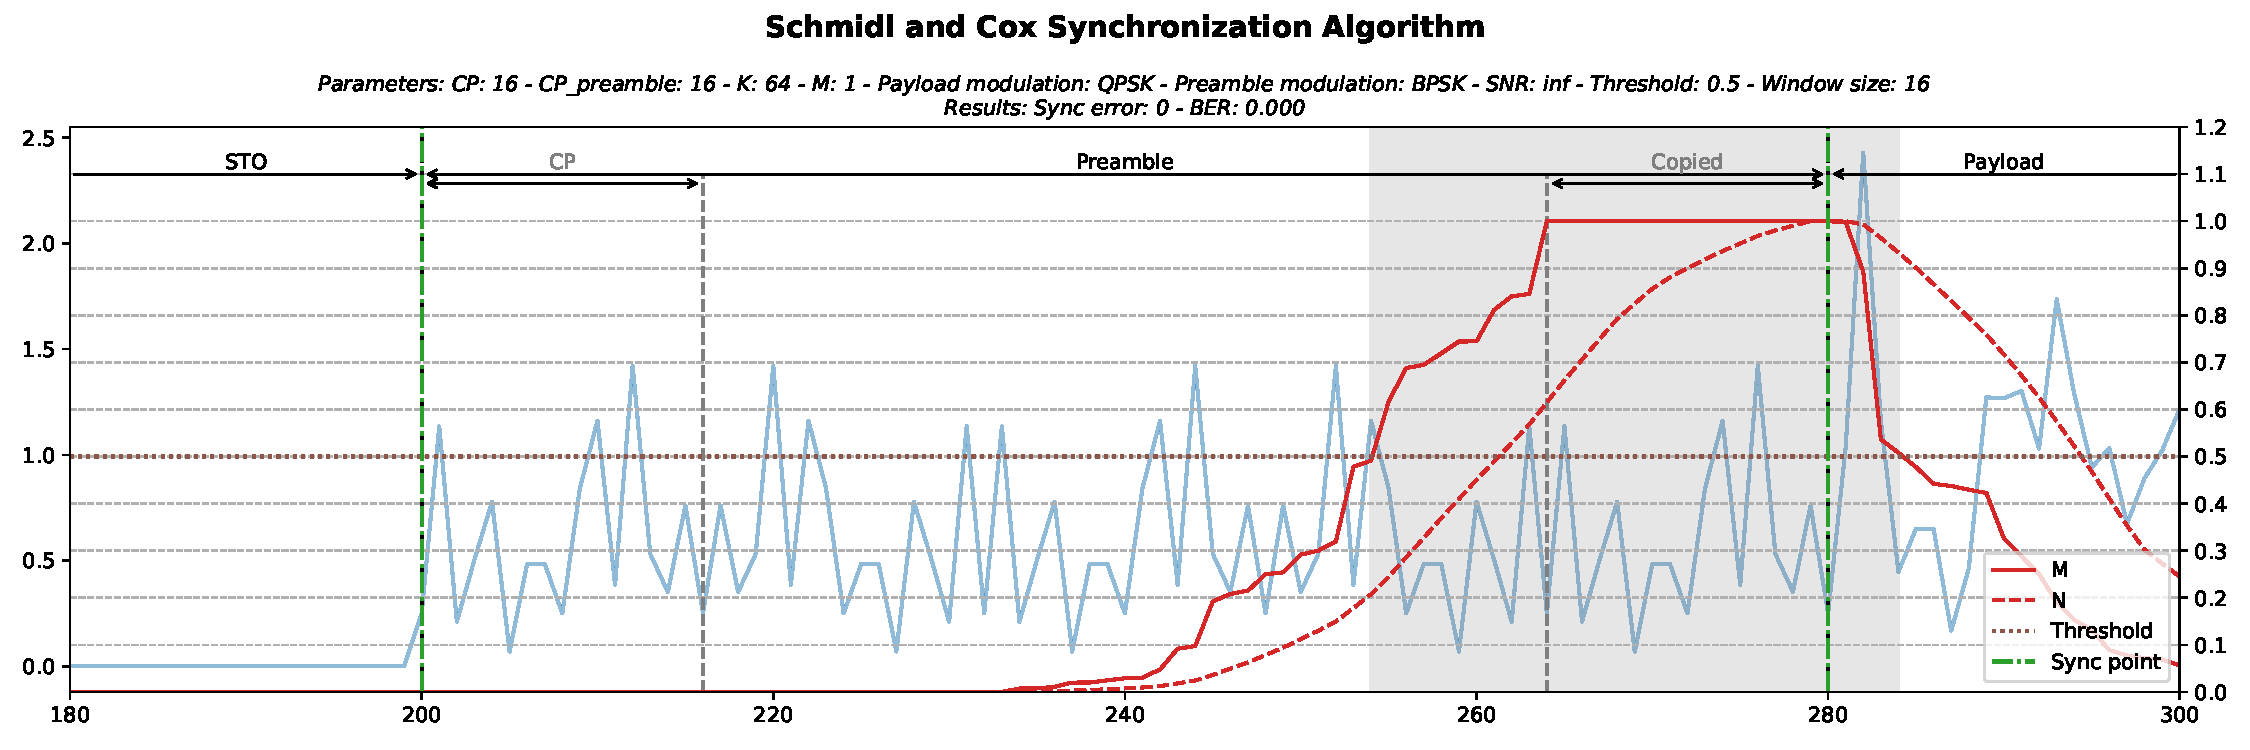
\includegraphics[width=\textwidth]{plots/sc_sync_cp16.pdf}
    \end{figure}
    \begin{figure}
        \centering
        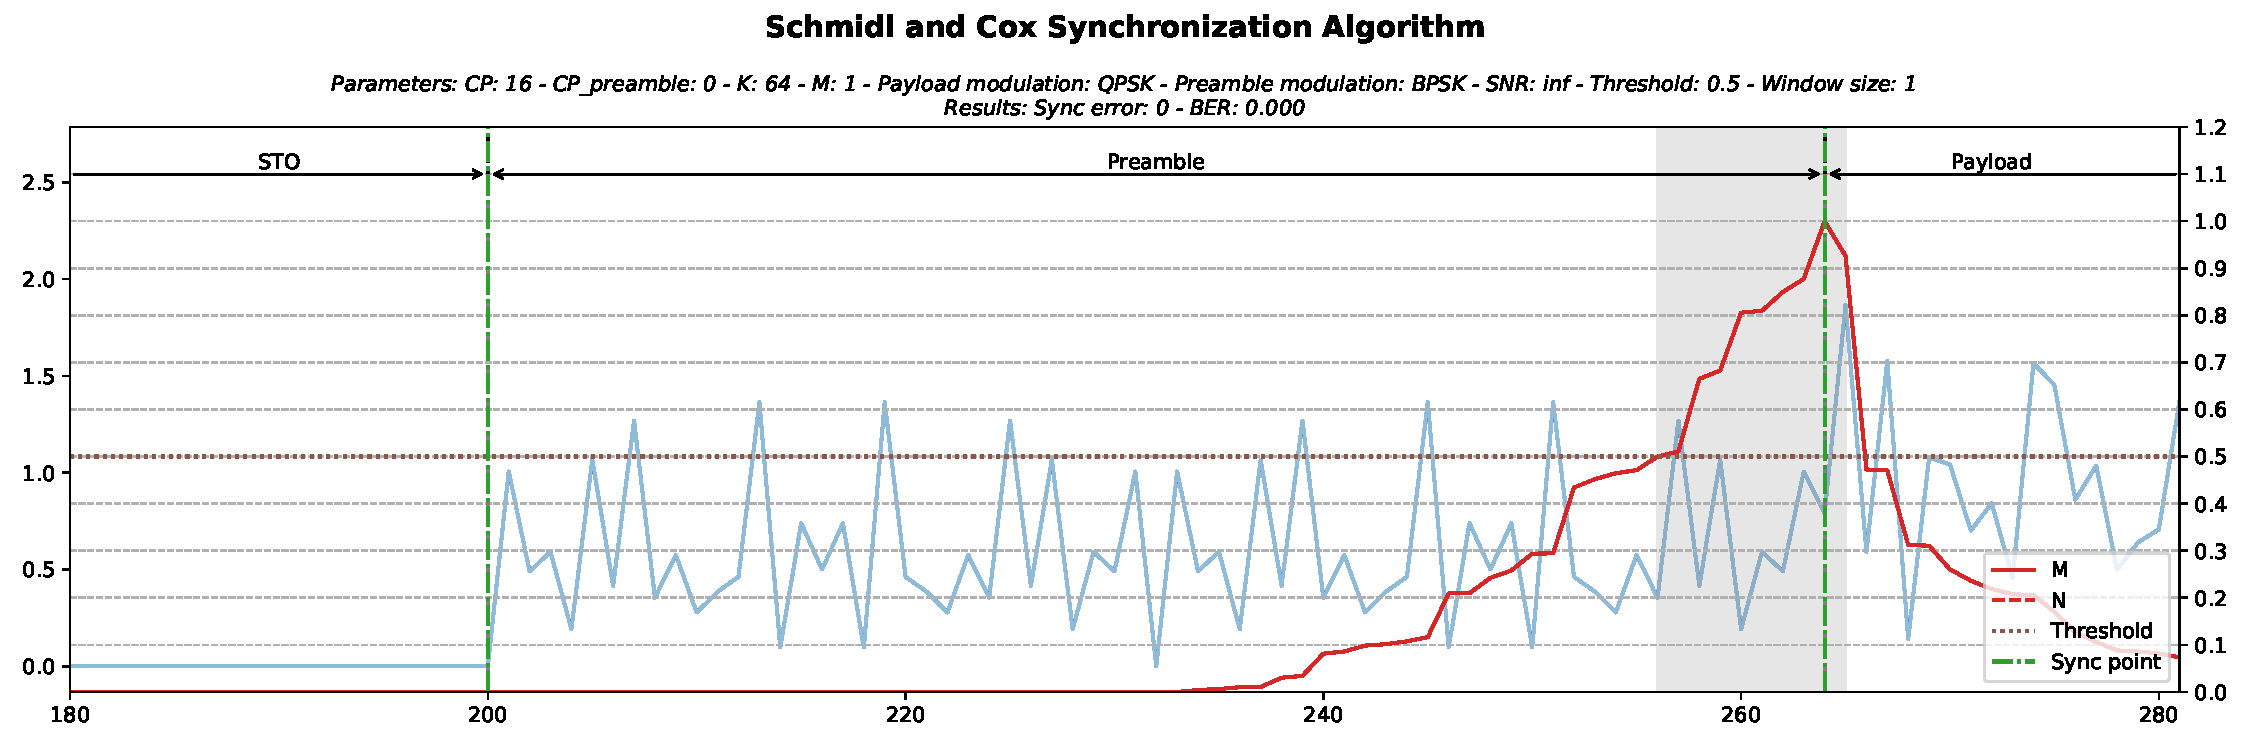
\includegraphics[width=\textwidth]{plots/sc_sync_nocp.pdf}
    \end{figure}
}

\frame{
    \frametitle{Theoretical Simulation - CDF of synchronization error}
    \begin{figure}
        \centering
        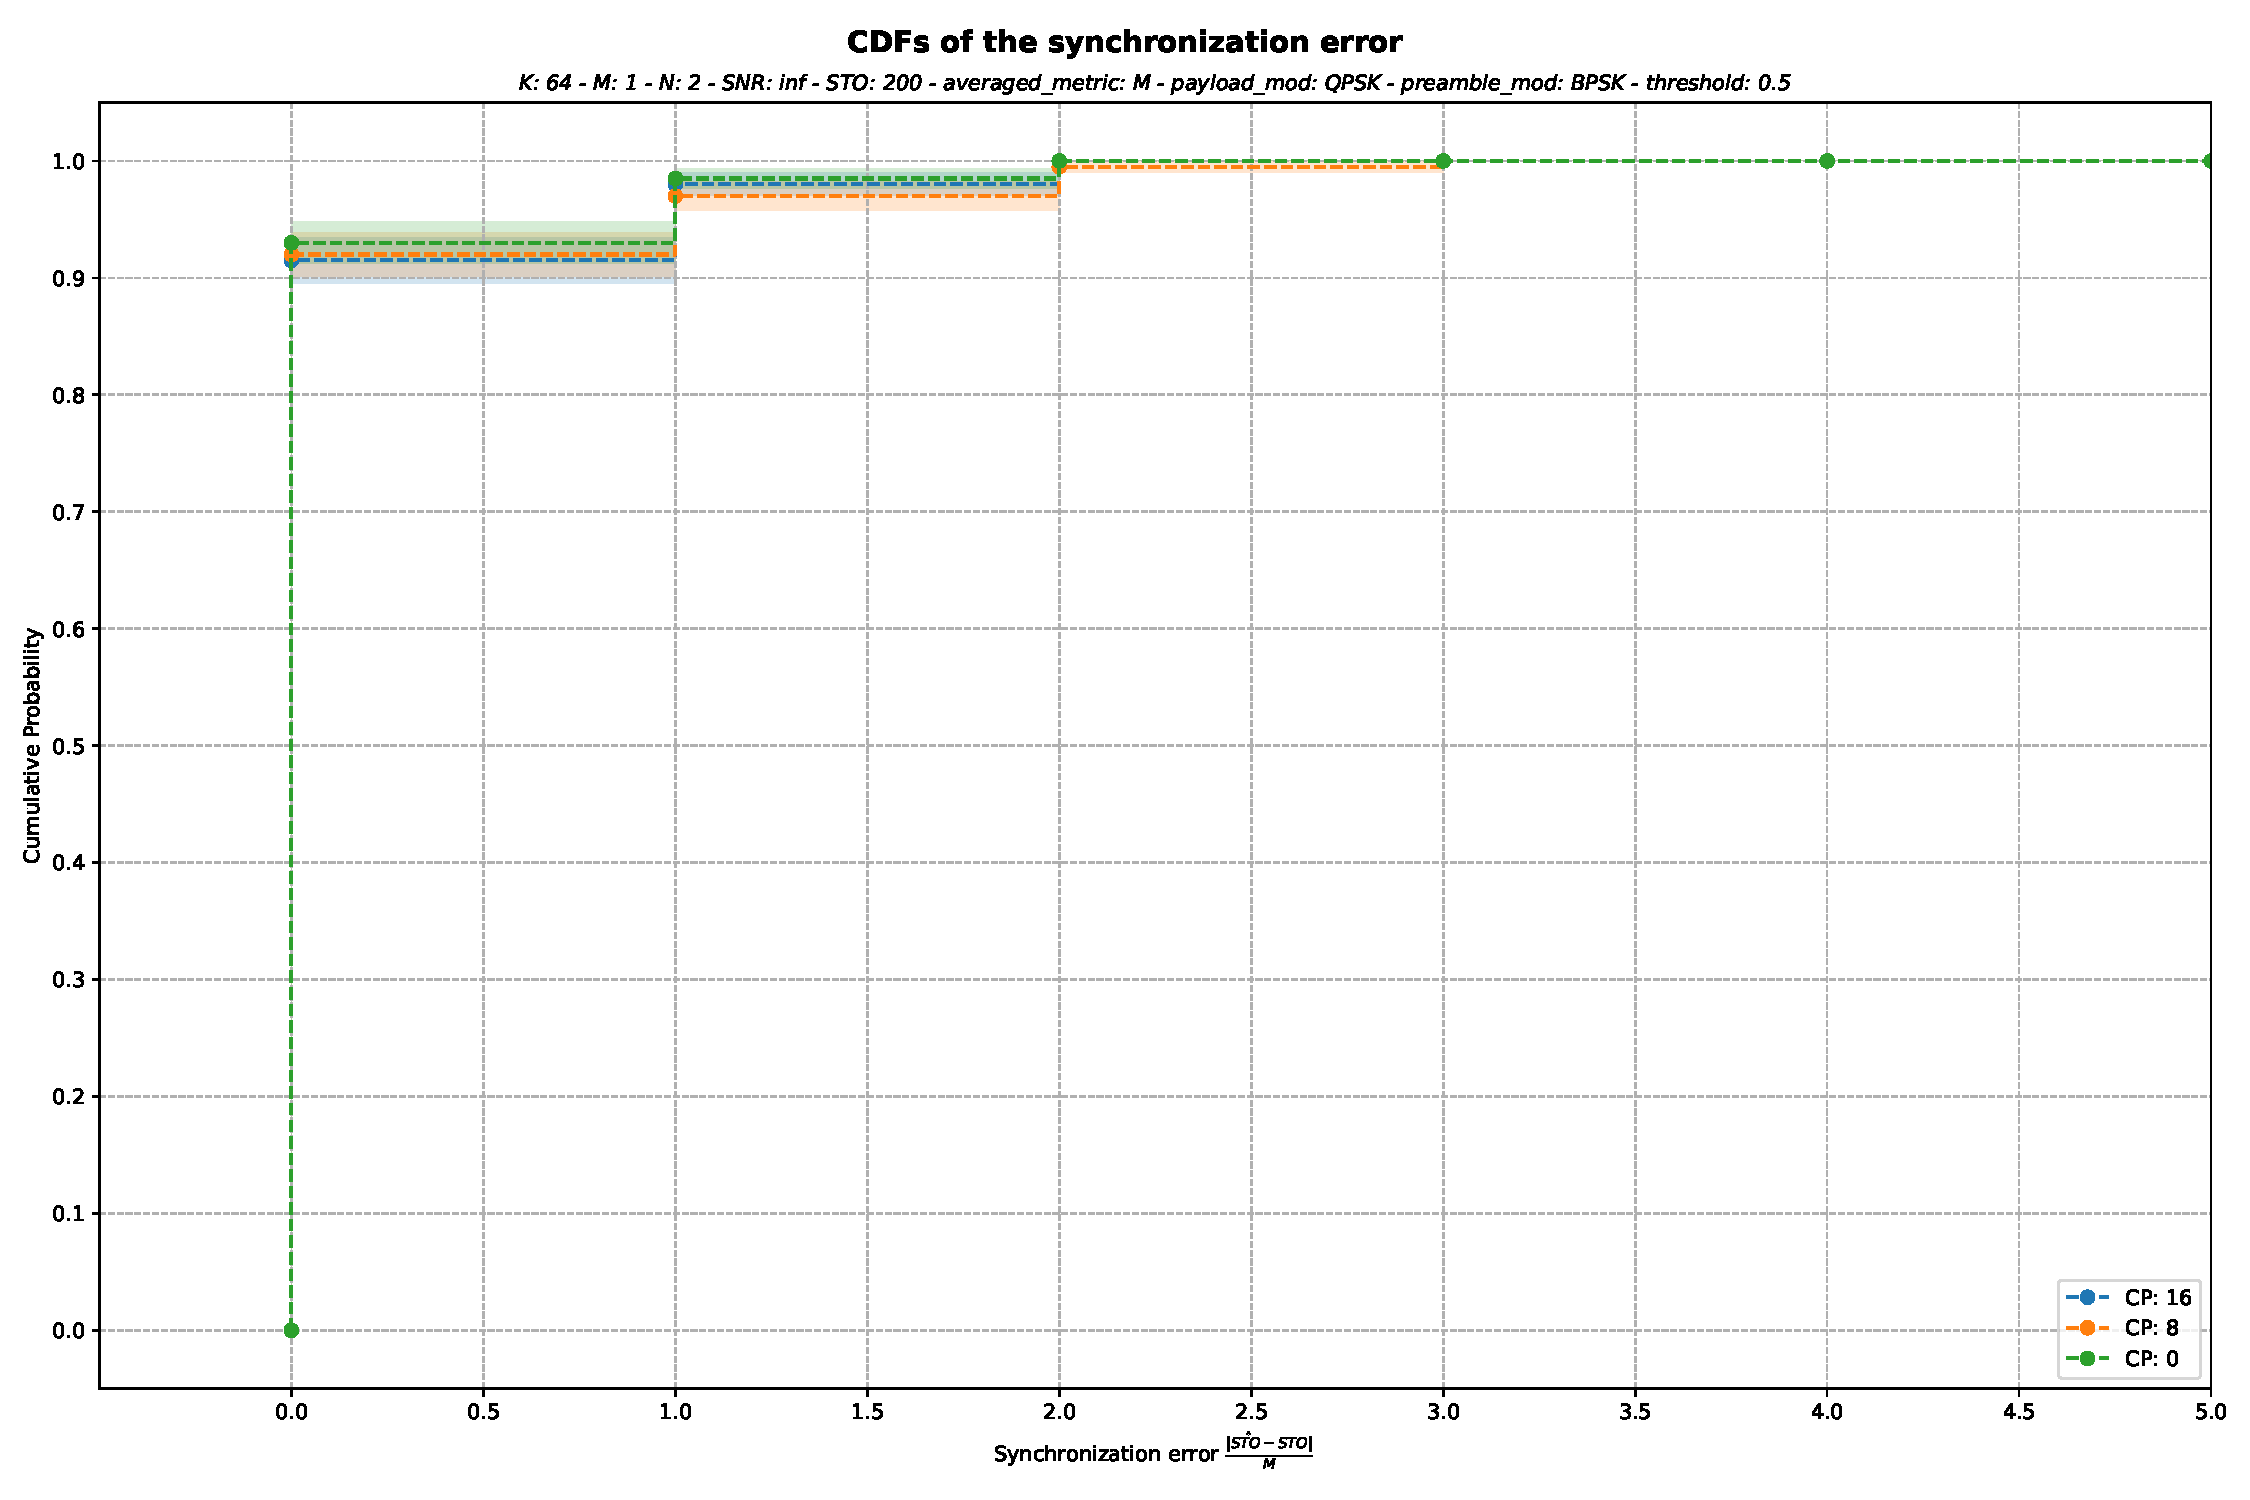
\includegraphics[width=\textwidth]{plots/sc_cdf_cp.pdf}
    \end{figure}
}

\frame{
    \frametitle{Theoretical Simulation - CDF of synchronization error}
    \begin{figure}
        \centering
        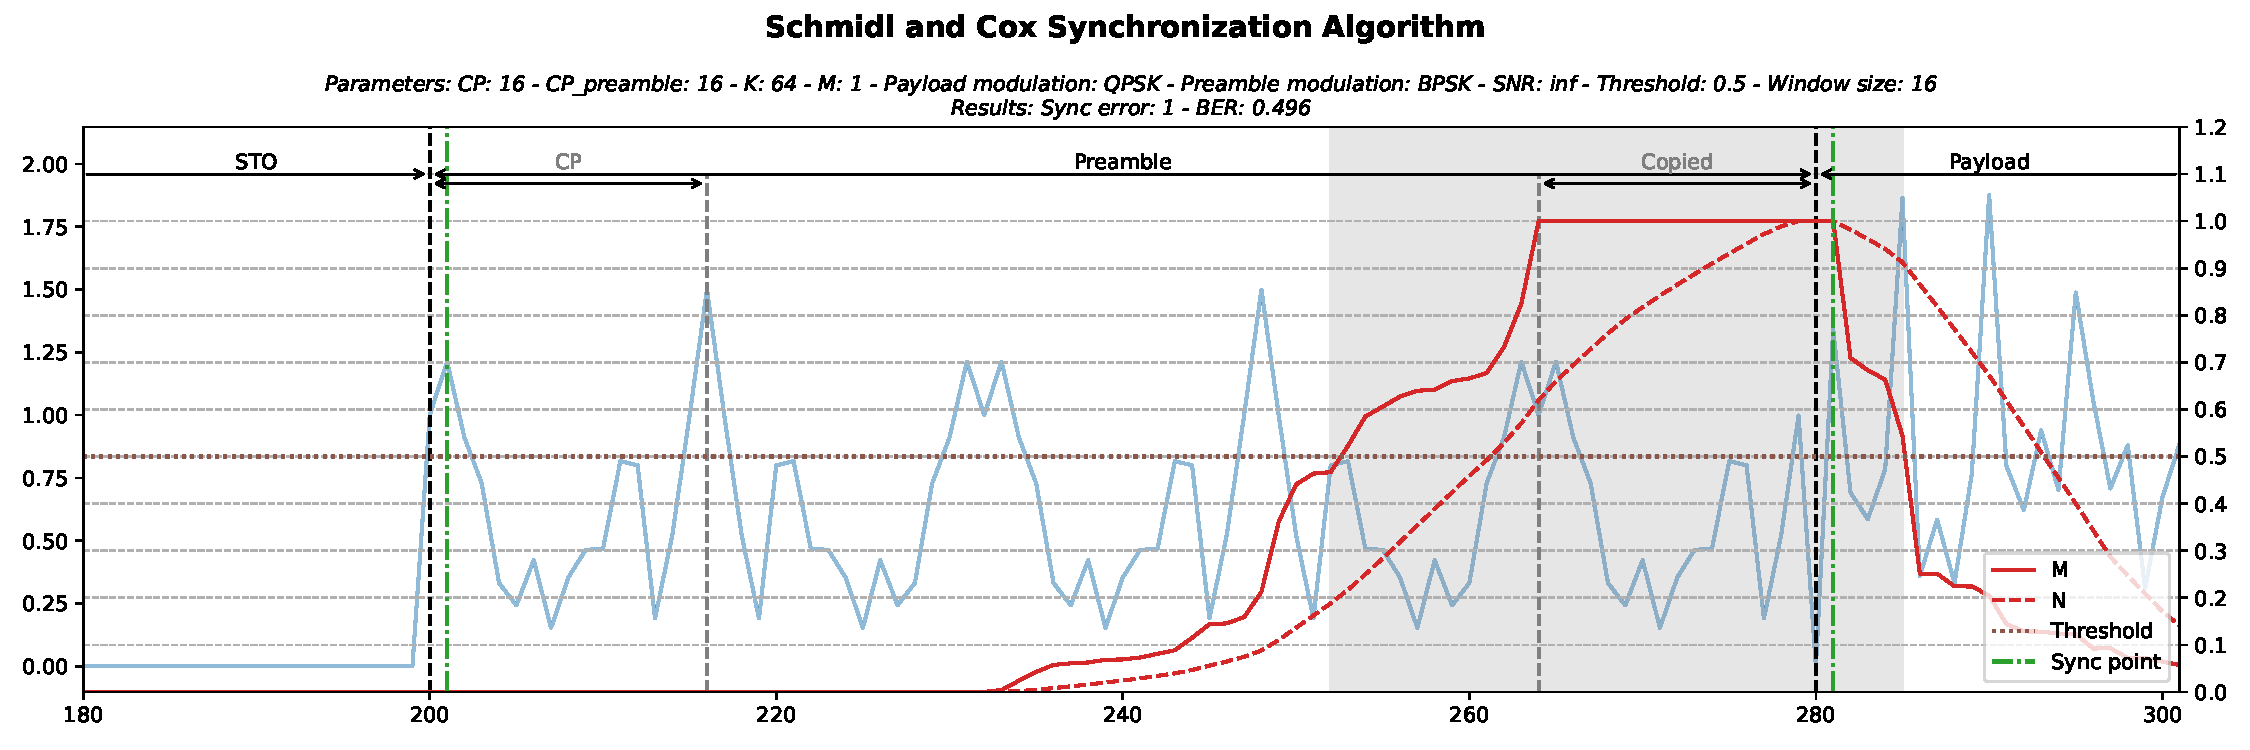
\includegraphics[width=\textwidth]{plots/sc_sync_cp16_ko_2051842398.pdf}
    \end{figure}
}

\frame{
    \frametitle{Theoretical Simulation - CDF of synchronization error}
    \begin{figure}
        \centering
        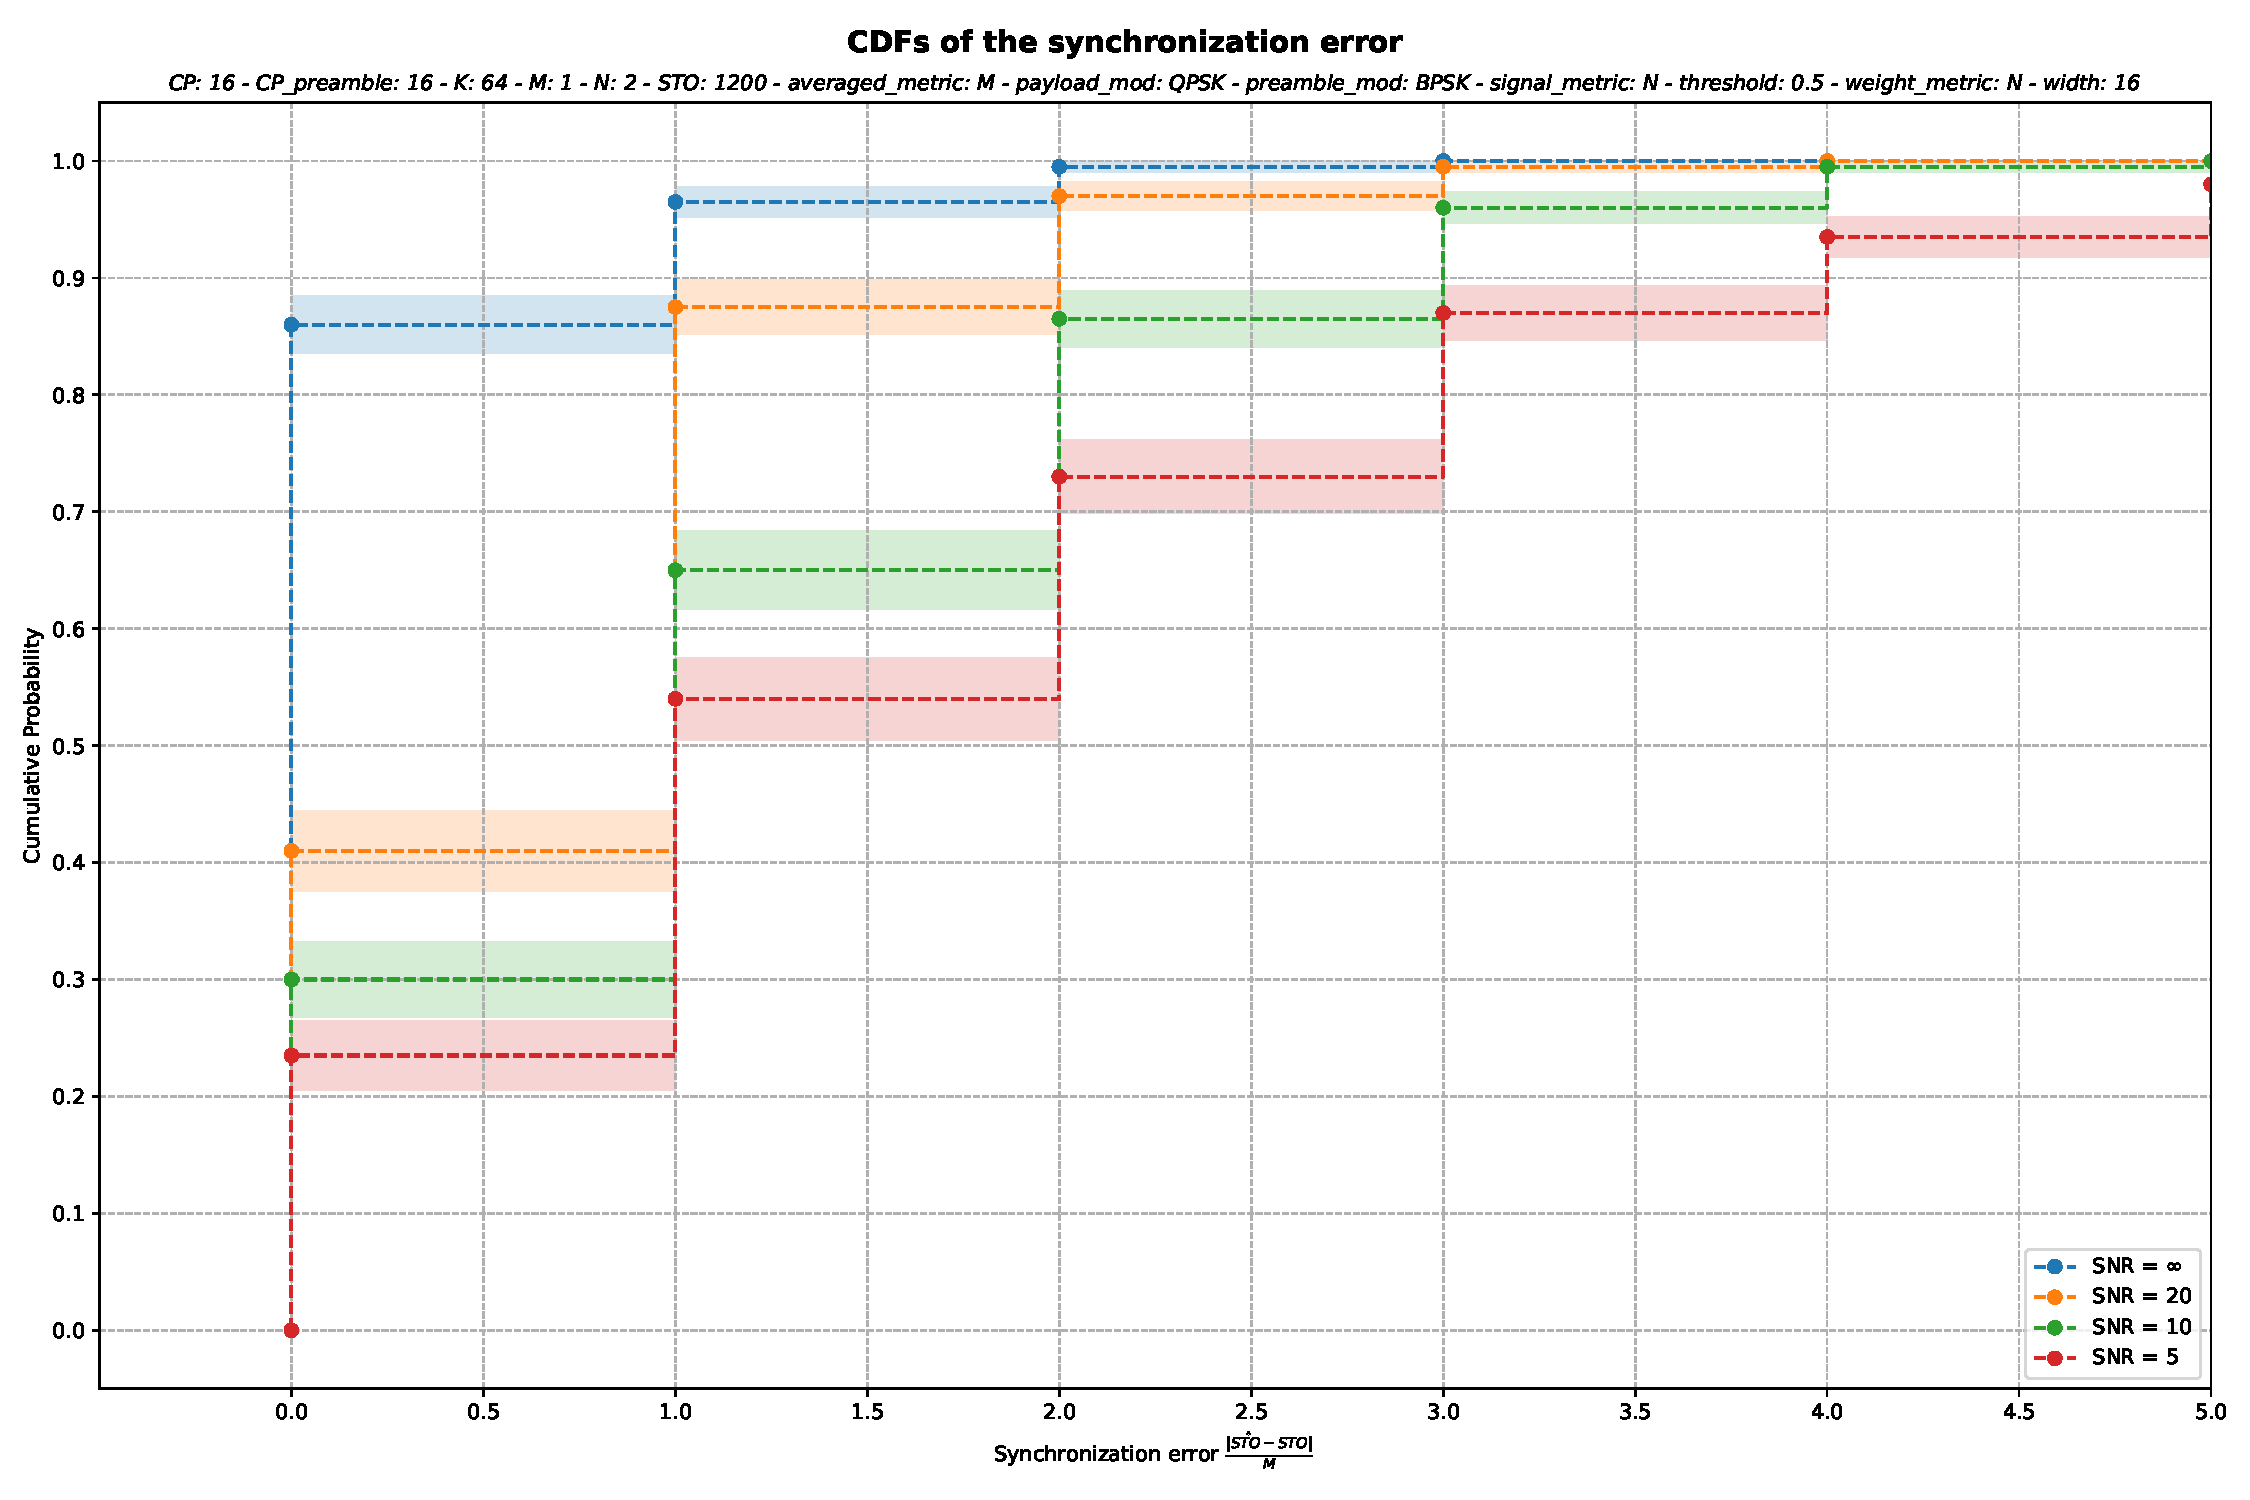
\includegraphics[width=\textwidth]{plots/sc_cdf_snr.pdf}
    \end{figure}
}

\frame{
    \frametitle{Theoretical Simulation - CDF of synchronization error}
    \begin{figure}
        \centering
        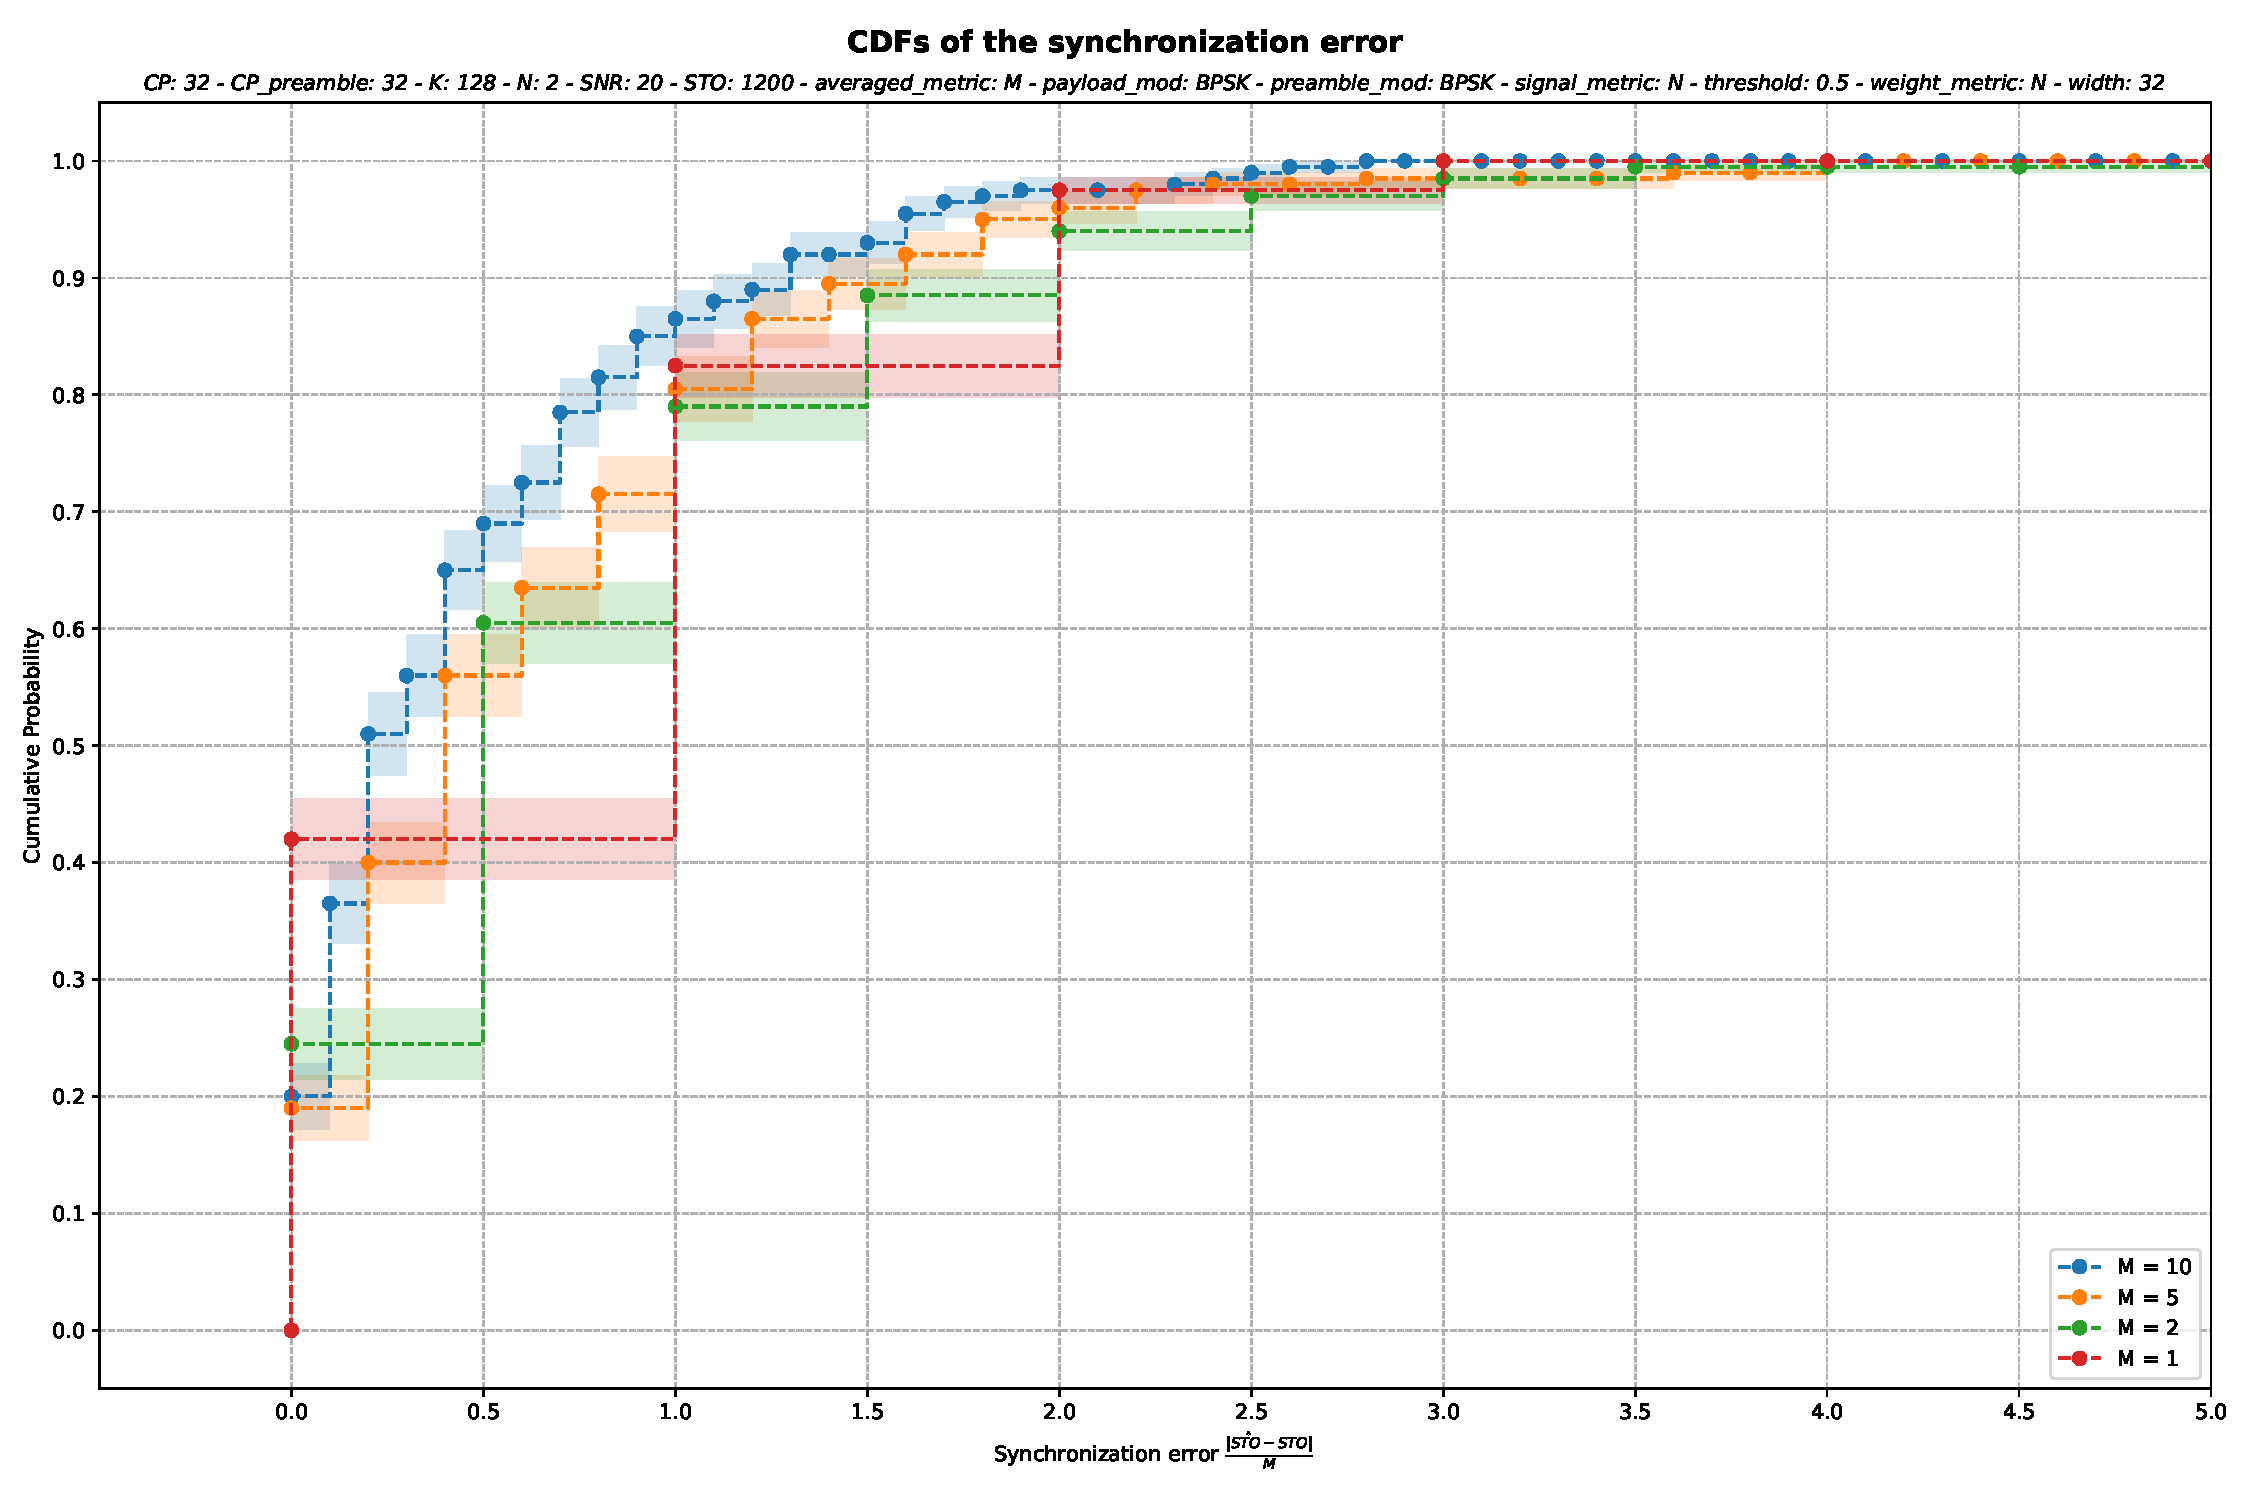
\includegraphics[width=\textwidth]{plots/sc_cdf_m.pdf}
    \end{figure}
}


%%%%%%%%%%%%%%%%%%%%%%%%%%%%
% PART 3: Doctorate thesis %
%%%%%%%%%%%%%%%%%%%%%%%%%%%%


\end{document}